\documentclass[../main.tex]{subfiles}
\begin{document}

\section*{第1問}

% Source: handwritten.pdf 第1問．
{\bf [解]}
点Aを始点とする位置ベクトルを小文字で表す．仮定より
\begin{align}
  \boldsymbol{c}\cdot(\boldsymbol{c}-\boldsymbol{b})&=0,\\
  \boldsymbol{d}\cdot(\boldsymbol{d}-\boldsymbol{b})&=0,\\
  \boldsymbol{b}\cdot(\boldsymbol{d}-\boldsymbol{c})&=0.
\end{align}
$\boldsymbol{m}=\dfrac{\boldsymbol{c}+\boldsymbol{d}}{2}$だから
\begin{align}
  \overrightarrow{AM}\cdot\overrightarrow{CD}
  &=\dfrac{1}{2}(\boldsymbol{c}+\boldsymbol{d})\cdot(\boldsymbol{d}-\boldsymbol{c})\\
  &=\dfrac{1}{2}(|\boldsymbol{d}|^2-|\boldsymbol{c}|^2)\\
  &=\dfrac{1}{2}(\boldsymbol{b}\cdot\boldsymbol{d}-\boldsymbol{b}\cdot\boldsymbol{c})=0.
\end{align}
よって$AM\perp CD$である．$AB\perp CD$でもあるから，平面ABMは直線CDと垂直である．
\begin{figure}[H]
  \begin{center}
    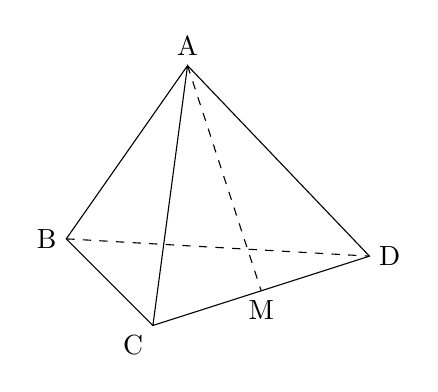
\begin{tikzpicture}[scale=1.1]
      \coordinate (A) at (1.4,3);\coordinate (B) at (0,1);\coordinate (C) at (1,0);\coordinate (D) at (3.5,.8);\coordinate (M) at (2.25,.4);
      \draw (A)--(B)--(C)--(D)--(A)--(C);\draw[dashed] (B)--(D) (A)--(M);
      \node[above] at (A){A};\node[left] at (B){B};\node[below left] at (C){C};\node[right] at (D){D};\node[below] at (M){M};
    \end{tikzpicture}
  \end{center}
  \caption{四面体ABCDと辺CDの中点M}
\end{figure}
\newpage

\section*{第2問}

% Source: handwritten.pdf 第2問．
まず三角形APBを形成するから，Pが直線$\mathrm{AB}:y=-\dfrac{1}{2}x+1$上に存在しないことは常にみたされる．
% 原稿p.3冒頭の直線ABの式をそのまま転記．問題のA(0,1)，B(0,2)とは整合しないため要確認．
$\angle APB=\theta$とする．ABを直径とする円
\begin{align}
  C:\quad x^2+\left(y-\dfrac{3}{2}\right)^2=\dfrac{1}{4}
\end{align}
と$y=x$が交わるか調べる．中心$(0,\dfrac{3}{2})$と$y=x$の距離は
\begin{align}
  \ell=\dfrac{|\dfrac{3}{2}|}{\sqrt{1+1}}=\dfrac{3}{2\sqrt{2}}>\dfrac{1}{2}
\end{align}
だから交わらない．よって$0\leqq\theta<\dfrac{\pi}{2}$であり，この区間で$\tan\theta$は広義単調増加関数である．
$\overrightarrow{PA}=(-x,1-x)$，$\overrightarrow{PB}=(-x,2-x)$より
\begin{align}
  \tan\theta&=\dfrac{|{-x(2-x)+x(1-x)}|}{x^2+(1-x)(2-x)}\\
  &=\dfrac{x}{2x^2-3x+2}\\
  &=\dfrac{1}{2(x+\dfrac{1}{x})-3}\leqq\dfrac{1}{4-3}=1.
\end{align}
最後は$x>0$に対する相加相乗平均の不等式を用いた．等号成立は$x=1$のときである．したがって求める最大値は
\begin{align}
  \max\theta=\dfrac{\pi}{4}.
\end{align}
\begin{figure}[H]
  \begin{center}
    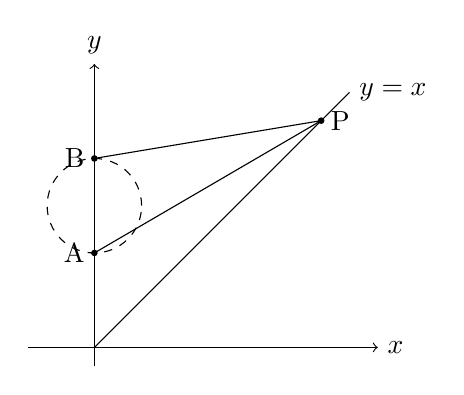
\begin{tikzpicture}[scale=1.2]
      \draw[->] (-.7,0)--(3,0) node[right]{$x$};\draw[->] (0,-.2)--(0,3) node[above]{$y$};
      \draw[dashed] (0,1.5) circle (.5);\draw (0,0)--(2.7,2.7) node[right]{$y=x$};
      \draw (0,1)--(2.4,2.4)--(0,2);
      \fill (0,1) circle (1pt) node[left]{A};\fill (0,2) circle (1pt) node[left]{B};\fill (2.4,2.4) circle (1pt) node[right]{P};
    \end{tikzpicture}
  \end{center}
  \caption{円Cと直線$y=x$上の点P}
\end{figure}
\newpage

\section*{第3問}

% Source: handwritten.pdf 第3問．
% 原稿p.4の見出しは「第4問」だが，内容は乙第3問に対応する．
$c=\cos x$，$s=\sin x$と略記する．まず
\begin{align}
  S=\int_0^\pi\sin x\,dx=2.
\end{align}
$y=\sin x$と$y=a\cos x$の交点の$x$座標を$\alpha$とすると，$0<\alpha<\dfrac{\pi}{2}$で
\begin{align}
  \sin\alpha=a\cos\alpha.
\end{align}
また
\begin{align}
  T&=\int_0^\alpha\sin x\,dx+\int_\alpha^{\pi/2}a\cos x\,dx\\
  &=1-\cos\alpha+a(1-\sin\alpha).
\end{align}
$S:T=3:1$より
\begin{align}
  0&=1-3\cos\alpha+3a(1-\sin\alpha).
\end{align}
$a=\dfrac{\sin\alpha}{\cos\alpha}$を代入して
\begin{align}
  0&=(1-3\cos\alpha)\cos\alpha+3\sin\alpha(1-\sin\alpha),\\
  3&=\cos\alpha+3\sin\alpha.
\end{align}
$t=\tan\dfrac{\alpha}{2}$とおけば
\begin{align}
  \cos\alpha=\dfrac{1-t^2}{1+t^2},\qquad \sin\alpha=\dfrac{2t}{1+t^2},
\end{align}
だから
\begin{align}
  3(1+t^2)&=1-t^2+6t,\\
  4t^2-6t+2&=0,\\
  (2t-1)(t-1)&=0.
\end{align}
$0<t<1$より$t=\dfrac{1}{2}$．したがって
\begin{align}
  a=\tan\alpha=\dfrac{2t}{1-t^2}=\dfrac{1}{1-\dfrac{1}{4}}=\dfrac{4}{3}.
\end{align}
\paragraph{解2}
$a=\tan\alpha$，$0<\alpha<\dfrac{\pi}{2}$だから
\begin{align}
  \sin\alpha=\dfrac{a}{\sqrt{a^2+1}},\qquad \cos\alpha=\dfrac{1}{\sqrt{a^2+1}}.
\end{align}
これらを$S:T=3:1$の式に代入しても$a=\dfrac{4}{3}$を得る．
\begin{figure}[H]
  \begin{center}
    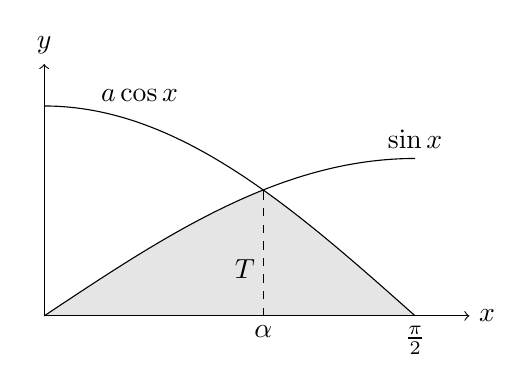
\begin{tikzpicture}[xscale=3,yscale=2]
      \fill[gray!20] (0,0)--plot[domain=0:.9273,samples=50](\x,{sin(\x r)})--plot[domain=.9273:1.5708,samples=50](\x,{4*cos(\x r)/3})--cycle;
      \draw[->] (0,0)--(1.8,0) node[right]{$x$};\draw[->] (0,0)--(0,1.6) node[above]{$y$};
      \draw plot[domain=0:1.5708,samples=60](\x,{sin(\x r)}) node[above]{$\sin x$};
      \draw plot[domain=0:1.5708,samples=60](\x,{4*cos(\x r)/3});\node[right] at (.2,1.4){$a\cos x$};
      \draw[dashed] (.9273,0) node[below]{$\alpha$}--(.9273,.8);\node[below] at (1.5708,0){$\frac{\pi}{2}$};\node at (.85,.3){$T$};
    \end{tikzpicture}
  \end{center}
  \caption{二つの曲線と$x$軸で囲まれる領域}
\end{figure}
\newpage

\section*{第4問}

% Source: handwritten.pdf 第4問．
$AB=a$，$AC=b$，$BC=\sqrt{3}$とし，外心をOとする．鋭角三角形なのでOは三角形の内部にある．$OB=OC=1$より
\begin{align}
  \angle BOC=\dfrac{2\pi}{3},\qquad \angle BAC=\dfrac{\pi}{3}.
\end{align}
余弦定理によって
\begin{align}
  3&=a^2+b^2-2ab\cdot\dfrac{1}{2}=a^2+b^2-ab,\\
  b&=\dfrac{a\pm\sqrt{12-3a^2}}{2}.
\end{align}
% 原稿の「複号負はb<0」を転記．sqrt(3)<a<2ではこの符号判定は成立せず，要確認．
$1<a<2$より負号の場合は$b<0$となるので不適．したがって
\begin{align}
  b=\dfrac{a+\sqrt{12-3a^2}}{2}.
\end{align}
\begin{figure}[H]
  \begin{center}
    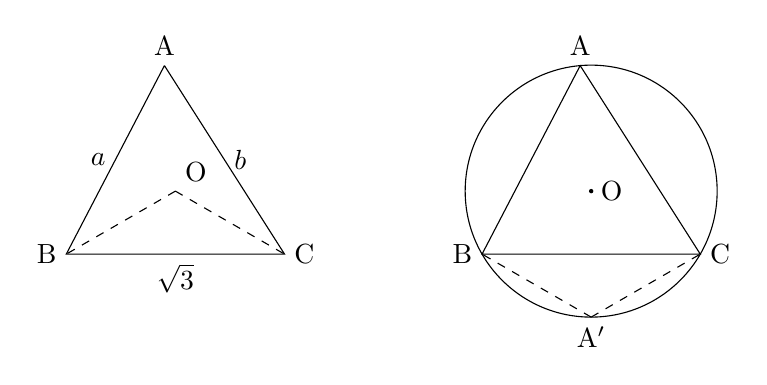
\begin{tikzpicture}[scale=1.6]
      \coordinate (O) at (0,0);\coordinate (B) at (210:1);\coordinate (C) at (330:1);\coordinate (A) at (95:1);
      \draw (A)--(B) node[midway,left]{$a$}--(C) node[midway,below]{$\sqrt{3}$}--(A) node[midway,right]{$b$};
      \draw[dashed] (O)--(B) (O)--(C);\node[above right] at (O){O};\node[above] at (A){A};\node[left] at (B){B};\node[right] at (C){C};
      \begin{scope}[xshift=3.3cm]
        \draw (0,0) circle (1);\draw (95:1)--(210:1)--(330:1)--cycle;\draw[dashed] (270:1)--(210:1) (270:1)--(330:1);
        \node[above] at (95:1){A};\node[below] at (270:1){$\mathrm{A}'$};\node[left] at (210:1){B};\node[right] at (330:1){C};\fill (0,0) circle (.5pt) node[right]{O};
      \end{scope}
    \end{tikzpicture}
  \end{center}
  \caption{三角形ABCの外心と円周角}
\end{figure}
\newpage

\section*{第5問}

% Source: handwritten.pdf 第5問．
\begin{enumerate}
  \item $a_n=3^{2^n}-1$とおく．$a_n$が$2^{n+2}$で割り切れ，$2^{n+3}$で割り切れないことを帰納法で示す．
    $n=1$のとき$a_1=8=2^3$だから成立する．$n=k$で成立すると仮定する．
    \begin{align}
      a_{k+1}=(3^{2^k}+1)(3^{2^k}-1).
    \end{align}
    ここで
    \begin{align}
      3^{2^k}+1&\equiv 1^{2^k}+1\equiv0\pmod{2},\\
      3^{2^k}+1&\equiv(-1)^{2^k}+1\equiv2\pmod{4}.
    \end{align}
    よって第1因子は2で割り切れ，4で割り切れない．仮定より$a_{k+1}$は$2^{k+3}$で割り切れ，$2^{k+4}$で割り切れない．帰納法により示された．
  \item $m=A2^n$（$A$は奇数，$n\geqq1$）と表す．
    \begin{align}
      3^m-1&=(3^{2^n})^A-1=(a_n+1)^A-1\\
      &=a_n\left\{a_n^{A-1}+\binom{A}{1}a_n^{A-2}+\cdots+\binom{A}{A-2}a_n+A\right\}.
    \end{align}
    中括弧内は奇数だから，(1)より$3^m-1$は$2^{n+2}$で割り切れ，$2^{n+3}$で割り切れない．したがって必要な条件は
    \begin{align}
      A2^n\leqq n+2.
    \end{align}
    $n\geqq3$では$A2^n\geqq n+3$である．実際，$n=3$では$A2^3\geqq8\geqq6$であり，$A2^k\geqq k+3$なら
    \begin{align}
      A2^{k+1}\geqq2(k+3)\geqq k+4
    \end{align}
    だから帰納法で従う．よって$n\geqq3$は不適．
    $n=1$では$2A\leqq3$より$A=1$，$m=2$．$n=2$では$4A\leqq4$より$A=1$，$m=4$．以上より
    \begin{align}
      m=2,4.
    \end{align}
\end{enumerate}
\newpage

\section*{第6問}

% Source: handwritten.pdf 第6問．
球および箱をすべて区別して考える．すべての場合の数は$(2n)^n$であり，どの箱にも球が2個以上入らない場合の数は
\begin{align}{}_{2n}P_n=(2n)(2n-1)\cdots(n+1).
\end{align}
したがって
\begin{align}
  p_n&=\prod_{k=n+1}^{2n}\dfrac{k}{2n},\\
  \log p_n&=\sum_{k=n+1}^{2n}\log\dfrac{k}{2n}.
\end{align}
区分求積法より
\begin{align}
  \lim_{n\to\infty}\dfrac{\log p_n}{n}
  &=2\int_{1/2}^1\log x\,dx\\
  &=2\left[x(\log x-1)\right]_{1/2}^1\\
  &=\log2-1.
\end{align}
\newpage

\end{document}
